\section{V7}
\subsection{Cortex M3 Instruction Set}
\begin{multicols}{2}  
\subsubsection{Thumb-2 Instruction Set}
\begin{tabular}{l l}
    Ziel&-Erhöht die Code-Dichte\\
        &  -Mehr Leistung\\ 
  Cortex M3 Processor  & 1.25 DMIPS / MHz\\ 
\end{tabular} 

\begin{minipage}{\textwidth}
\subsection{Logikstruktur des Cortex-M Prozessor}
\begin{tabular}{ll} 
    Sourceoperanden& Rn, Rm \\ 
    Destinationsoperand& Rd  \\ 
\end{tabular} \\
Ein \textit{Barrel-Shifter} vereinfacht Berechnungen,\newline
da Multiplikationen einfacher realisiert werden können.
\end{minipage}
\end{multicols}

\begin{multicols}{2}
     \subsection{Instruction Pipelining}
     \begin{minipage}{\linewidth}
         MAC = Memory Access Calculator\\
         Load Store Architektur
     \end{minipage}   
     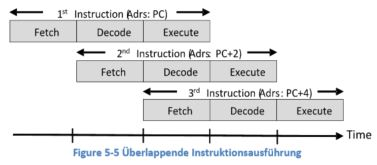
\includegraphics[width=\linewidth]{images/pipelining}
     
    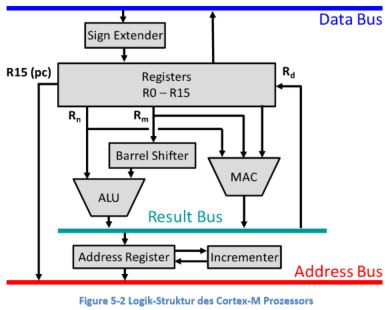
\includegraphics[width=0.8\linewidth]{images/logikstrukturcortex}
\end{multicols}

\subsection{Anwendungen}
\begin{multicols}{3}
    \begin{minipage}{\linewidth}
       \subsubsection{Cortex-M0/M0+ / M1}  
       einfaches I/O Handling 
    \end{minipage}
    
    \begin{minipage}{\linewidth}
        \subsubsection{Cortex-M3}   
        Komplexe Datenverarbeitung\newline
        anspruchsvolle Applikationenen
    \end{minipage}

    \begin{minipage}{\linewidth}
        \subsubsection{Cortex-M4}   
        DSP-Funktionalität\newline
        Floating Point Support
    \end{minipage}
\end{multicols}
    
\subsection{Assembly-Language Syntax}
\begin{tabular}{llll}
    \textbf{Lable}  &\textbf{OpCode}  &\textbf{Operand}  & \textbf{Comment} \\ 
    L1& ADD &R0,R1,\#5  & Replace R0 by sum of R1 and 5 \\ 
    FUNC& MOV &R0,\#100  & this sets R0 to value 100 \\  
    &BX&LR& this is a function return\\
\end{tabular} 
\begin{tabular}{|ll}
    \textbf{Lable}& optional  \\ 
    \textbf{OpCode}& spezifiziert den Befehl \\ 
    \textbf{Operand}& Parameter  \\ 
    \textbf{Comment}&  optionale Beschriebung\\ 
\end{tabular} 
\\
\begin{multicols}{2}
    \begin{minipage}{\linewidth}
        \subsection{Unified Assembler Language (UAL)}
        Syntax für ARM und Thumb Instructionen.\\
        Die meisten Instruktionen arbeiten mit Registern\\
        \textbf{BSP}\newline
            \begin{tabular}{lll}
                MOV&R2,\#100  &;R2=100,Direkte Zuweisung  \\ 
                LDR&R2,[R1]  &;R2= den Wert von R1  \\ 
                ADD&R2,R0    &;R2=R2+R0  \\ 
                ADD&R2,R0,R  &;R2=R0+R1  \\ 
            \end{tabular} 
    \end{minipage}
    
    \begin{minipage}{0.8\linewidth}
        \subsubsection{Register List}
        \begin{tabular}{lll}
            Norm. Form&{reglist}  &;{R1,R2...Rn}  \\ 
            PUSH& {LR} & ;save LR on stack\\ 
            POP&  {LR}&  ;remove from stack; place in LR\\  
            PUSH& {R1-R3,LR} & ;save R1,R2,R3; return address\\  
            POP& {R1-R3,PC} &;restore R1,R2,R3 and return \\ 
        \end{tabular} 
    \end{minipage}
\end{multicols}
\clearpage

\subsection{Addressing}
\begin{multicols}{2}
    \begin{minipage}{\linewidth}
    \subsubsection{Immediate Adressing}
       Der Datenwert ist unmittelbar in der Instruktion erhalten. Daher kein zusätzlicher Speicherzugriff erforderlich\newline
       Form: \# imm\newline
       \begin{tabular}{lll}
          MOV & R0,\# 100&;R0=100, immediate addressing \\ 
        \end{tabular} 
    \end{minipage}
    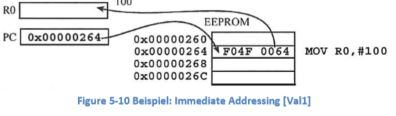
\includegraphics[width=0.9\linewidth]{images/immediateAddressing}    
\end{multicols}   


\begin{multicols}{2}
    \begin{minipage}{\linewidth}
    \subsubsection{Indirect Addressing}
        Bei der indirekten Adressierung sind mehrere Speicherzugriffe erforderlich.\newline
        Form: [Rn]\newline
           \begin{tabular}{lll}
              LDR & R0,[R1]&;R0=value pointed to by R1 \\ 
            \end{tabular} \\
        Ein Register enthält irgendwie eien Zeiger auf dieses Register\newline
        \textbf{R1 wird nicht verändert}
     \end{minipage}
     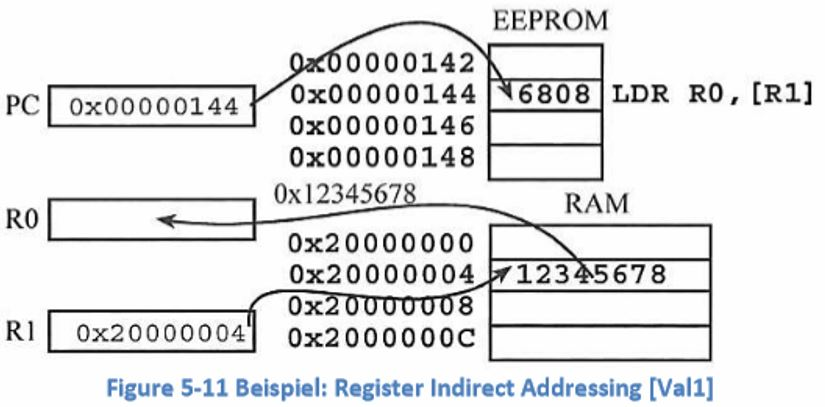
\includegraphics[width=0.9\linewidth]{images/indirectAddressing}    
\end{multicols} 


\begin{multicols}{2}
    \begin{minipage}{\linewidth}
    \subsubsection{Register Addressing with Displacment}
        Dasselbe nur wierd hier dem Wert R0 noch \# 4 hinzugefügt\newline
        R1 bleibt weiterhin unverändert.\newline
        Form: [Rn,\# imm]\newline
        \begin{tabular}{lll}
            LDR & R0,[R1,\# 4]&;R0=word pointed to by R1+4 \\ 
        \end{tabular} \\
    \end{minipage}
    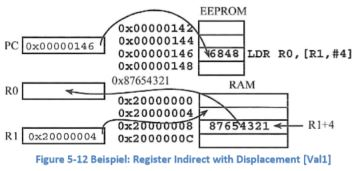
\includegraphics[width=0.9\linewidth]{images/AddressingDisplacment}    
\end{multicols} 

\subsubsection{Register Indirect with Index}
Form: [Rn,Rm]\newline
\begin{tabular}{lll}
   LDR &R0,[R1,R2]  &;R0= word pointed to by R1+R2 \\ 
\end{tabular} 

\subsubsection{Register Indirect with shifted Index}
Form: [Rn,Rm,LSL \# imm]\newline
\begin{tabular}{lll}
    LDR&R0,[R1,R2;LSL \#2]  &;R0= word pointed to by R1+4*R2  \\ 
\end{tabular} 

\subsubsection{Register Indirect with Pre-index}
Form: [Rn,\# offset]!\newline
\begin{tabular}{lll}
   LDR & R0,[R1,\#4]! &;first R1=R1+4, then R0= word pointed to by R1  \\ 
\end{tabular} 

\subsubsection{Register Indirect with Post-index}
Form: [Rn],\# offset\newline
\begin{tabular}{lll}
    LDR& R0,[R1],\#4  &;R0= word pointed to by R1, then R1=R1+4  \\ 
\end{tabular} 

\subsubsection{PC-relativ}
PC wird als Pointer verwendet.
Form: lable\newline
\begin{tabular}{lll}
    B   &Location   &;jump to Location\\ 
    BL  &Subroutine &;call Subroutine, Rücksprungadresse wird gespeichert\\ 
\end{tabular} 

\subsubsection{Speicher- und I/O-Zugriffe}
\begin{multicols}{2}
    \begin{minipage}{\linewidth}
    Es benötigt immer zwei Instruktionen um auf Daren im RAM oder I/O zuzugreifen.
    \rightarrow PC-Relative Addressierung wird verwendet
    \begin{enumerate}
        \item Erstellt Zeuger auf das Objekt
        \item Greift über den Zeiger Indirekt auf den Speicher zu
    \end{enumerate}
    \begin{tabular}{lll}
        LDR   &R1,Count   &;R1 points to variable Count\\ 
        LDR  &R0,[R1] &;R0= value pointed to by R1\\ 
    \end{tabular} 
\end{minipage}

    \includegraphics[width=\linewidth]{images/AddressingRAM}   
\end{multicols}





















